\documentclass[12pt,a4paper]{article}

\usepackage[a4paper,top=1in,bottom=1in,left=1in,right=1in]{geometry}
\usepackage{amsmath}
\usepackage{amssymb}
\usepackage{graphicx}
\usepackage{booktabs}
\usepackage{subcaption}
\usepackage{float}
\usepackage{tikz}
\usetikzlibrary{positioning,arrows.meta}
\usepackage{fancyhdr}
\usepackage{microtype}
\usepackage{hyperref}
\hypersetup{colorlinks=true, linkcolor=blue, urlcolor=blue}
\captionsetup{hypcap=false}

\graphicspath{{../results/}{results/}}

\setlength{\parindent}{0pt}
\setlength{\parskip}{0pt}
\setlength{\abovedisplayskip}{2pt}
\setlength{\belowdisplayskip}{2pt}
\setlength{\abovedisplayshortskip}{1pt}
\setlength{\belowdisplayshortskip}{1pt}
\setlength{\emergencystretch}{1em}
\hfuzz=2pt
\setlength{\headheight}{15pt}

\pagestyle{fancy}
\fancyhf{}
\fancyhead[L]{Pool Ball Detection and Recognition}
\fancyhead[R]{M. H. Alaskandrani}
\fancyfoot[C]{\thepage}
\renewcommand{\headrulewidth}{0.4pt}

\title{\vspace{-1.4cm}\textbf{Pool Ball Detection and Recognition}}
\author{\textbf{Mahmoud Hatem Alaskandrani}\\[0.25em]
Trinity College Dublin / The American University in Cairo}
\date{\today}

\begin{document}

\maketitle
\thispagestyle{fancy}

\begin{abstract}
This report presents a two-stage computer vision pipeline for localising and recognising pool balls. Stage~1 fuses multi-channel CIELAB Canny edges, applies a dynamic pocket and netting mask, and detects circles with Hough, a 40-pixel physical NMS, and a raw-frame recovery path. Stage~2 uses 30/32-bin hue and saturation histograms, a 30/70 saturation-dominant distance, and a split-mask cue gate. Across the six tables the final system achieves Stage~1 precision, recall, and F1 of $0.911$, and Stage~2 recognition accuracy of $76.8\%$ on correctly localised balls.
\end{abstract}

\section{Introduction}

The task was to localise every pool ball on a rectified table image and classify it as one of the sixteen balls. The six test images contain strong shadows, uneven lighting, dense racks, solids, and stripes. I developed the pipeline through explicit experiments and retained an error analysis of the failures that remain. The repository is at \url{git@gitlab.scss.tcd.ie:csu33012-2627-group07/project07.git}.

\subsection{End-to-End Pipeline Overview}

Each image is warped into the $1434\times683$ metric frame. Stage~1 fuses Canny edges from the $L/a/b$ channels, applies a dynamic pocket and netting mask, and runs Hough Circles with 40-pixel minimum separation, a 22-pixel cushion margin, and 40-pixel NMS. A raw-frame recovery branch runs Standard Canny and Hough on the unwarped image, projects candidates through $\mathbf{H}$, and fuses them when they lie more than 30 pixels from every rectified detection. Stage~2 compares 30/32-bin hue and saturation histograms using a 30/70 distance and a split-mask cue gate, rejecting distances above $0.55$ (Figure~\ref{fig:pipeline}).

\begin{figure}[H]
\centering
\resizebox{0.97\linewidth}{!}{%
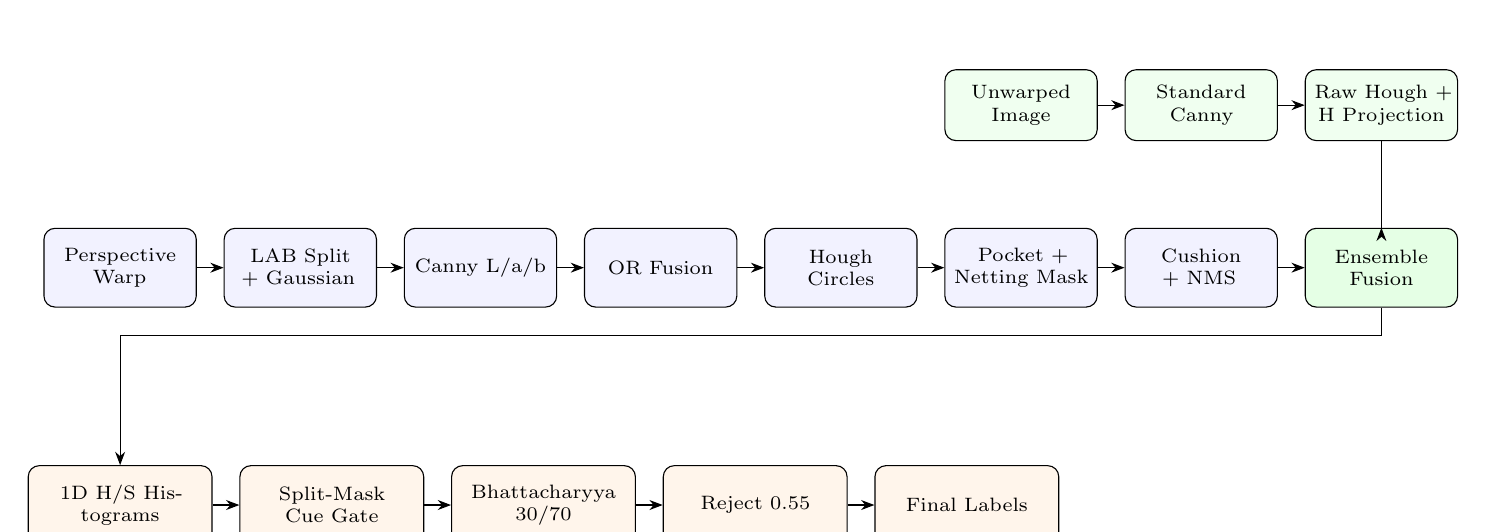
\begin{tikzpicture}[>=Stealth, node distance=0.28cm and 0.34cm,
 stage1/.style={draw, rounded corners, fill=blue!5, align=center, minimum height=1.0cm, text width=1.7cm, font=\scriptsize},
 stage2/.style={draw, rounded corners, fill=orange!8, align=center, minimum height=1.0cm, text width=2.1cm, font=\scriptsize},
 raw/.style={draw, rounded corners, fill=green!6, align=center, minimum height=0.9cm, text width=1.7cm, font=\scriptsize}]
% Stage 1 row
\node[stage1] (warp) {Perspective Warp};
\node[stage1,right=of warp] (lab) {LAB Split + Gaussian};
\node[stage1,right=of lab] (canny) {Canny L/a/b};
\node[stage1,right=of canny] (orfuse) {OR Fusion};
\node[stage1,right=of orfuse] (hough) {Hough Circles};
\node[stage1,right=of hough] (mask) {Pocket + Netting Mask};
\node[stage1,right=of mask] (nms) {Cushion + NMS};
\node[stage1, fill=green!10, right=of nms] (fusion) {Ensemble Fusion};
% Raw-frame recovery branch
\node[raw, above=1.1cm of mask] (unwarped) {Unwarped Image};
\node[raw, right=of unwarped] (rawcanny) {Standard Canny};
\node[raw, right=of rawcanny] (rawhough) {Raw Hough + H Projection};
% Stage 2 row
\node[stage2, below=2.0cm of warp] (hist) {1D H/S Histograms};
\node[stage2,right=of hist] (gate) {Split-Mask Cue Gate};
\node[stage2,right=of gate] (bhat) {Bhattacharyya 30/70};
\node[stage2,right=of bhat] (reject) {Reject 0.55};
\node[stage2,right=of reject] (labels) {Final Labels};
\draw[->] (warp)--(lab); \draw[->] (lab)--(canny); \draw[->] (canny)--(orfuse);
\draw[->] (orfuse)--(hough); \draw[->] (hough)--(mask); \draw[->] (mask)--(nms); \draw[->] (nms)--(fusion);
\draw[->] (unwarped)--(rawcanny); \draw[->] (rawcanny)--(rawhough);
\draw[->] (rawhough.south) |- (fusion.north);
\draw[->] (fusion.south) -- ++(0,-0.35) -| (hist.north);
\draw[->] (hist)--(gate); \draw[->] (gate)--(bhat); \draw[->] (bhat)--(reject); \draw[->] (reject)--(labels);
\end{tikzpicture}}
\caption{End-to-end pipeline architecture.}
\label{fig:pipeline}
\end{figure}
\vspace{-4pt}

\section{Stage 1: Ball Detection}

\subsection{Perspective rectification}

Each photograph is mapped by a planar homography from the four cushion corners into a $1434\times683$ metric frame matching the $1434\,\mathrm{mm}\times683\,\mathrm{mm}$ playing area, so one transformed pixel is one millimetre.

\subsection{Failed green-channel boost and adaptive thresholding}

To recover green balls I first boosted the RGB green channel by $1.5$ and applied adaptive Gaussian thresholding (block $15$, constant $2$). This failed because the green felt was boosted equally and its woven texture dominated the edge map; ball boundaries washed out.

\subsection{Failed HSV and single-channel lightness thresholding}

I then thresholded HSV with fixed ranges $H$ $35$--$85$, $S$ $40$--$255$, and $V$ $40$--$255$. Green balls $6$ and $14$ vanished because their hue and saturation overlap the felt. A single-channel lightness threshold also failed: shadows fragmented ball boundaries and dark balls could not be separated from the table. These failures motivated a multi-channel approach.

\begin{figure}[H]
\centering
\begin{subfigure}[b]{0.42\textwidth}
\centering
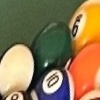
\includegraphics[width=\linewidth]{report_hsv_original.jpeg}
\caption{Region around the green ball.}
\end{subfigure}\hfill
\begin{subfigure}[b]{0.42\textwidth}
\centering

\includegraphics[width=\linewidth]{report_hsv_mask.jpeg}
\caption{Fixed HSV mask: green ball merges into felt.}
\end{subfigure}
\caption{Static HSV thresholding fails for green object balls: the green ball vanishes into the green felt.}
\label{fig:hsvfailure}
\end{figure}
\vspace{2pt}

\subsection{Successful multi-channel CIELAB edge fusion}

I split the rectified image into CIELAB, smoothed all channels with a $5\times5$ Gaussian ($\sigma=1.2$), and ran Canny independently: thresholds $45/95$ on $L$ and $35/85$ on $a$ and $b$. A logical OR fused the three edge maps, capturing both luminance silhouettes and colour boundaries that survive shadow. Figure~\ref{fig:labedges} shows the rectified Table~4 image and its fused edge map.

\begin{figure}[H]
\centering
\begin{subfigure}[b]{0.42\textwidth}
\centering
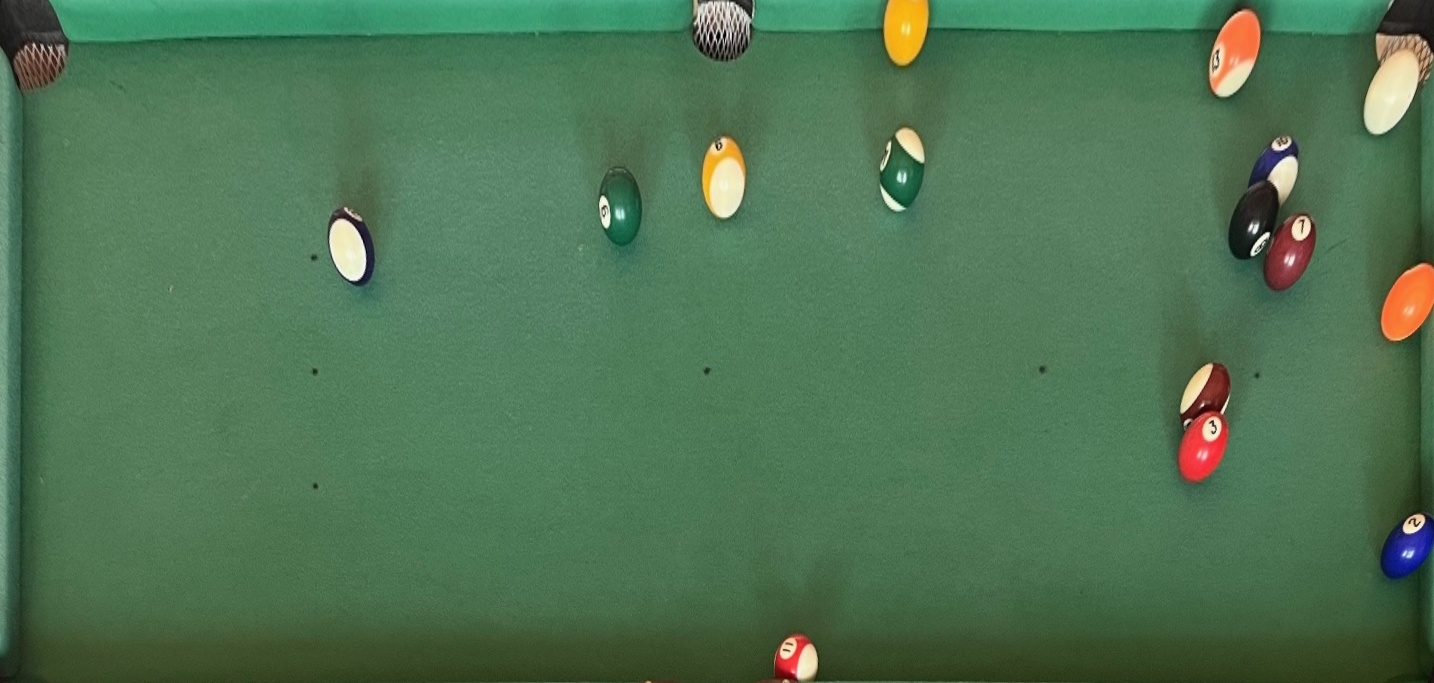
\includegraphics[width=\linewidth]{report_table4_warped.jpeg}
\caption{Rectified Table~4.}
\end{subfigure}\hfill
\begin{subfigure}[b]{0.42\textwidth}
\centering
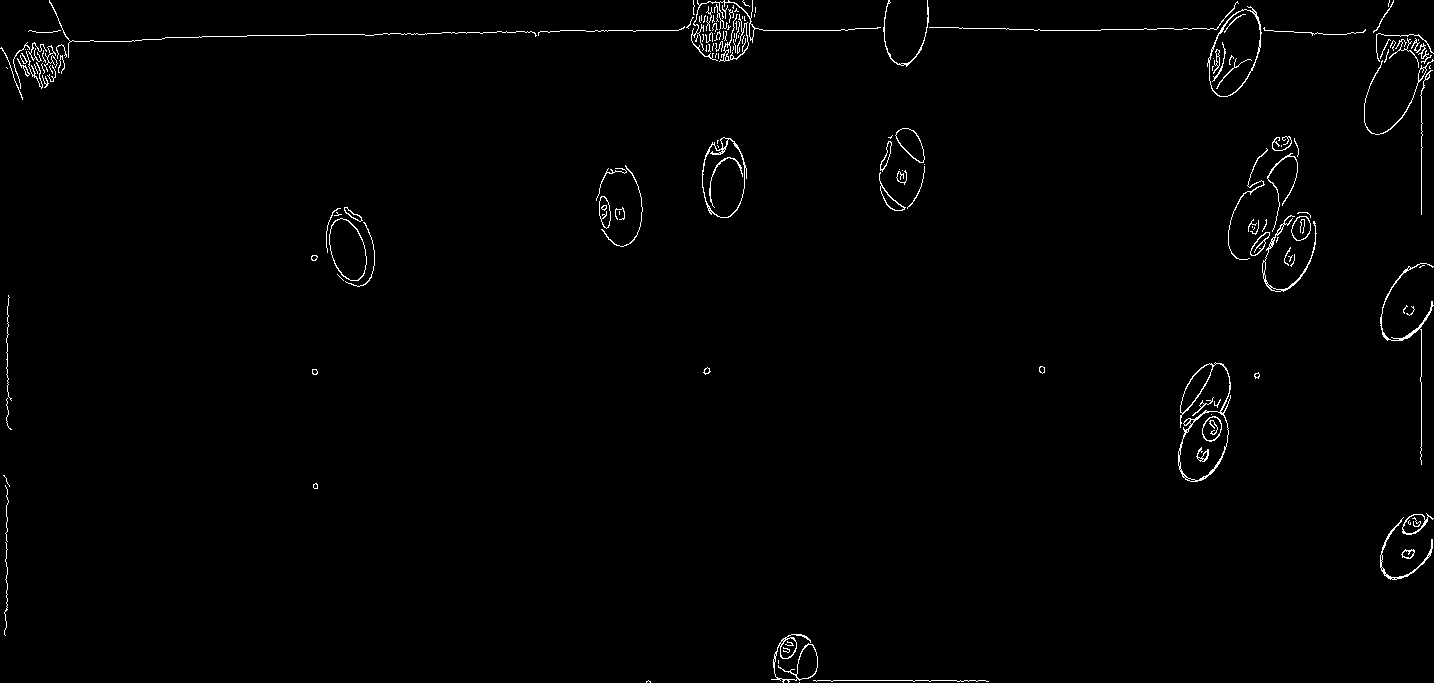
\includegraphics[width=\linewidth]{report_table4_edges.jpeg}
\caption{Gaussian-smoothed LAB Canny edge map.}
\end{subfigure}
\caption{Rectification and multi-channel LAB Canny edge fusion.}
\label{fig:labedges}
\end{figure}
\vspace{2pt}

\subsection{Dynamic pocket mask, netting mask, and physical NMS}

The fused map is passed to Hough with minDist $40$ and radius $19$--$24$. A blind $95$-pixel pocket rejection removed genuine corner balls, so I replaced it with a dynamic mask. For each pocket I thresholded a $120\times120$ region for dark holes ($L<35$) and bright brackets ($L>200$), dilated the LAB edges with a $15\times15$ kernel to capture netting, OR-ed the masks, restricted each to $70$ pixels, and dilated the combined mask with $13\times13$. A candidate is rejected only when its centre lies on this hole--bracket--netting mask. I kept a $22$-pixel cushion margin because $5$ pixels recovered far-edge balls but reintroduced rail shadows.

Hough occasionally returned intersecting peaks for one ball, so I enforce a $40$-pixel physical NMS. Zhang--Suen thinning removed almost nothing ($1.025$ pixels per skeleton pixel), and a $param2$ sweep made ghosts disappear only at $14$ while true balls fell from $83$ to $15$. I therefore added a raw-frame path: Canny and Hough on the unwarped image ($param2=14$, minDist $30$, radius $18$--$30$), projected through $\mathbf{H}$, and fused only if more than $30$ pixels from every rectified detection. This recovered three balls, raising TP from $79$ to $82$ and F1 from $0.893$ to $0.911$, with FP unchanged.

\section{Stage 2: Ball Recognition and Classification}

\subsection{Failed K-Means clustering}

I first tried $K=2$ K-Means on each ball mask and compared cluster colours with the references. It was slow and rotation-dependent: on a solid ball the clusters split the number and specular highlights rather than producing a stable stripe descriptor.

\subsection{Successful saturation-dominant histograms}

I switched to 1D histograms: 30 hue bins and 32 saturation bins from a 16-pixel circular mask, compared with the sixteen references by Bhattacharyya distance. A white stripe lowers saturation regardless of rotation, so I weight hue $0.30$ and saturation $0.70$ and reject distances above $0.55$:
\[
d = 0.30\,d_{\mathrm{hue}} + 0.70\,d_{\mathrm{sat}}.
\]
Tightening to $0.55$ removed circular rail shadows. The cue histogram overlapped green-felt reflections, so I added a split-mask gate: a 16-pixel centre for brightness and whiteness and a 21-pixel mask for overall paint. Centre value $>235$, centre saturation $<75$, and full saturation $<76$ excluded the purple $12$ and $9$ while retaining the cue; the Highlander rule selects the lowest full saturation.

Figure~\ref{fig:sathist} compares saturation histograms of solid ball~2 and striped ball~10. The solid ball peaks at high saturation; the white stripe creates a distinct low-saturation peak independent of rotation.

\begin{figure}[H]
\centering
\begin{subfigure}[b]{0.42\textwidth}
\centering
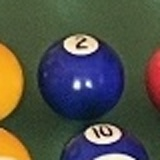
\includegraphics[width=0.32\linewidth]{crop_ball2.jpeg}\hfill
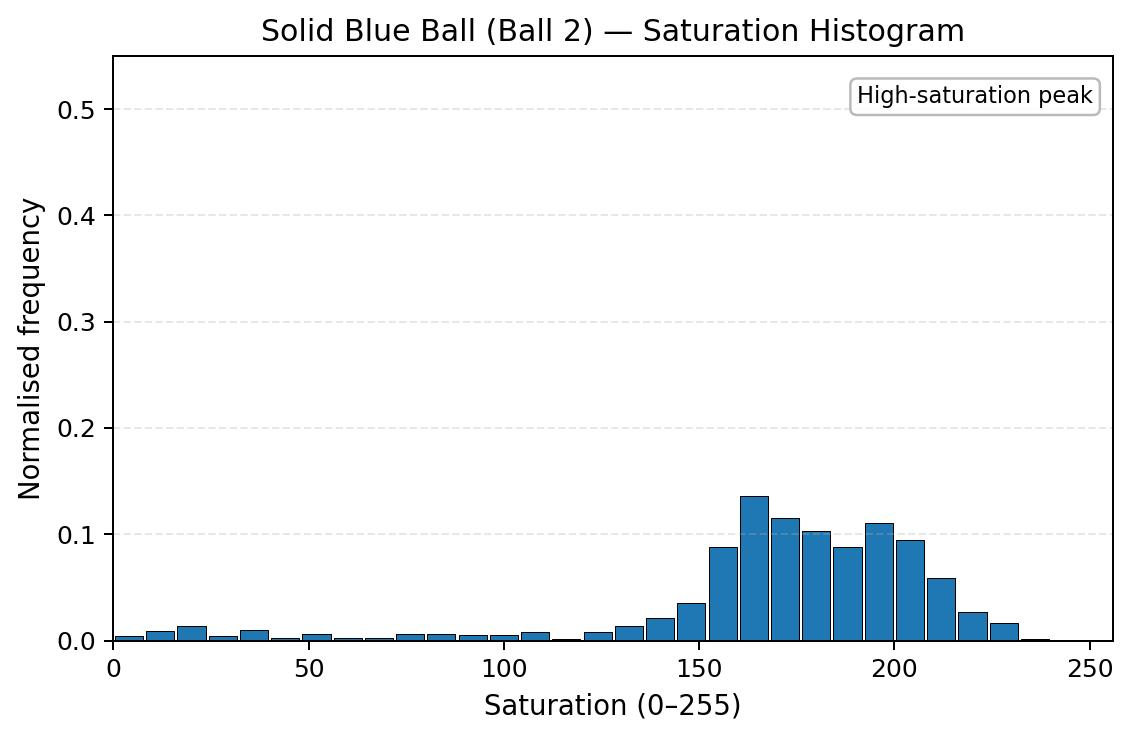
\includegraphics[width=0.64\linewidth]{report_hist_solid.jpeg}
\caption{Solid ball~2: high-saturation peak.}
\end{subfigure}\hfill
\begin{subfigure}[b]{0.42\textwidth}
\centering
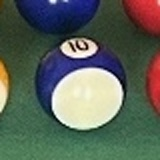
\includegraphics[width=0.32\linewidth]{crop_ball10.jpeg}\hfill
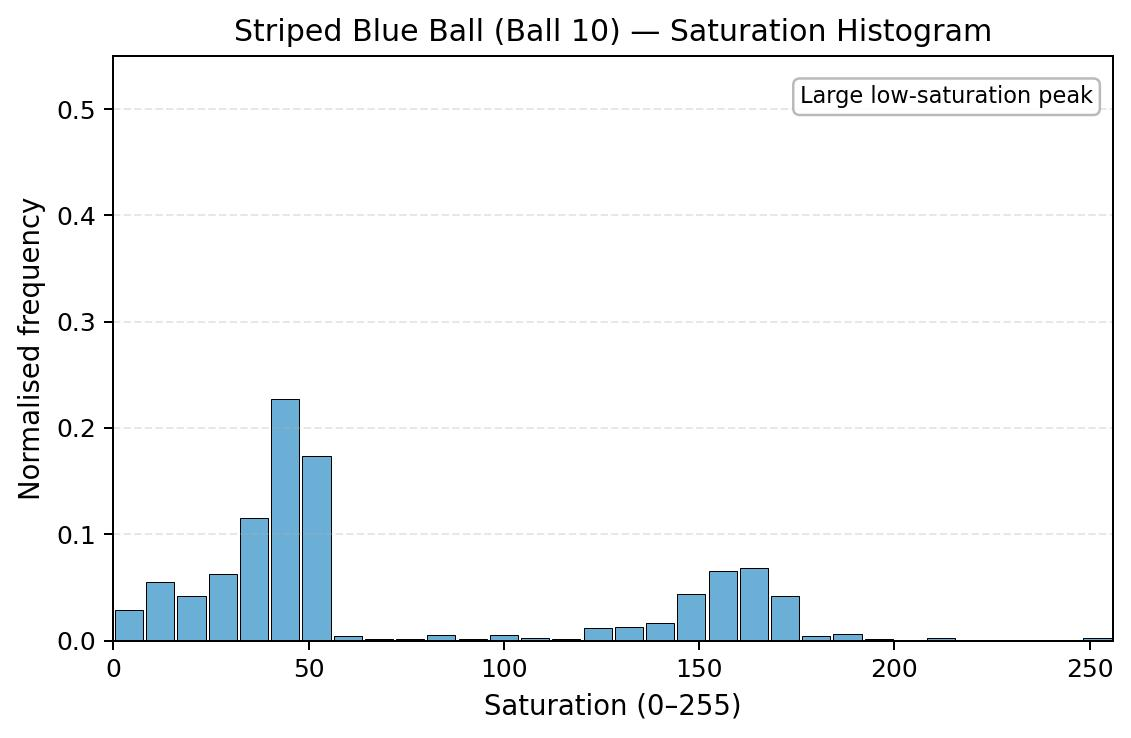
\includegraphics[width=0.64\linewidth]{report_hist_stripe.jpeg}
\caption{Striped ball~10: low-saturation peak from the white stripe.}
\end{subfigure}
\caption{Blue-ball comparison: each crop sits beside its 1D saturation histogram.}
\label{fig:sathist}
\end{figure}
\vspace{2pt}

\section{Results and Error Analysis}

\subsection{Stage 1: Detection Results}

Stage~1 uses one-to-one greedy matching within $21.5$ pixels, half the $43$-pixel diameter. A detected centre is a True Positive when its distance to an unmatched ground-truth centre satisfies
\[
\sqrt{(x_{\mathrm{det}}-x_{\mathrm{gt}})^2+(y_{\mathrm{det}}-y_{\mathrm{gt}})^2}\le 21.5\ \mathrm{px}.
\]
An unmatched detection is a False Positive and an unmatched ground-truth centre is a False Negative. Precision, recall, and F1 are
\[
\mathrm{Precision}=\frac{\mathrm{TP}}{\mathrm{TP}+\mathrm{FP}},\quad
\mathrm{Recall}=\frac{\mathrm{TP}}{\mathrm{TP}+\mathrm{FN}},\quad
\mathrm{F1}=2\cdot\frac{\mathrm{Precision}\cdot\mathrm{Recall}}{\mathrm{Precision}+\mathrm{Recall}}.
\]
Table~\ref{tab:stage1} reports per-table and overall metrics; overall precision, recall, and F1 are all $0.911$.

\begin{table}[H]
\centering
\caption{Stage~1 detection metrics after dynamic pocket masking.}
\label{tab:stage1}
\begin{tabular}{lcccccc}
\toprule
Image & TP & FP & FN & Precision & Recall & F1-score \\
\midrule
Table 1 & 13 & 0 & 3 & 1.000 & 0.812 & 0.897 \\
Table 2 & 15 & 2 & 1 & 0.882 & 0.938 & 0.909 \\
Table 3 & 16 & 0 & 0 & 1.000 & 1.000 & 1.000 \\
Table 4 & 14 & 2 & 1 & 0.875 & 0.933 & 0.903 \\
Table 5 & 13 & 2 & 1 & 0.867 & 0.929 & 0.897 \\
Table 6 & 11 & 2 & 2 & 0.846 & 0.846 & 0.846 \\
\midrule
Overall & 82 & 8 & 8 & 0.911 & 0.911 & 0.911 \\
\bottomrule
\end{tabular}
\end{table}

\subsection{Stage 2: Recognition Results}

Stage~2 accuracy is measured only over Stage~1 True Positives:
\[
\mathrm{Recognition\ Accuracy}=\frac{\text{correctly labelled Stage~1 TPs}}{\text{total Stage~1 TPs}}.
\]
A TP is wrong when its 30/70 weighted distance is closest to another reference or exceeds $0.55$. Across six tables, $63$ of $82$ correctly localised balls receive the correct label ($76.8\%$).

\begin{table}[H]
\centering
\caption{Stage~2 recognition accuracy on correctly localised balls.}
\label{tab:stage2}
\begin{tabular}{lccc}
\toprule
Image & Correct labels & True positives & Accuracy \\
\midrule
Table 1 & 10 & 13 & 0.769 \\
Table 2 & 10 & 15 & 0.667 \\
Table 3 & 12 & 16 & 0.750 \\
Table 4 & 13 & 14 & 0.929 \\
Table 5 & 10 & 13 & 0.769 \\
Table 6 & 8 & 11 & 0.727 \\
\midrule
Overall & 63 & 82 & 0.768 \\
\bottomrule
\end{tabular}
\end{table}

\begin{figure}[H]
\centering
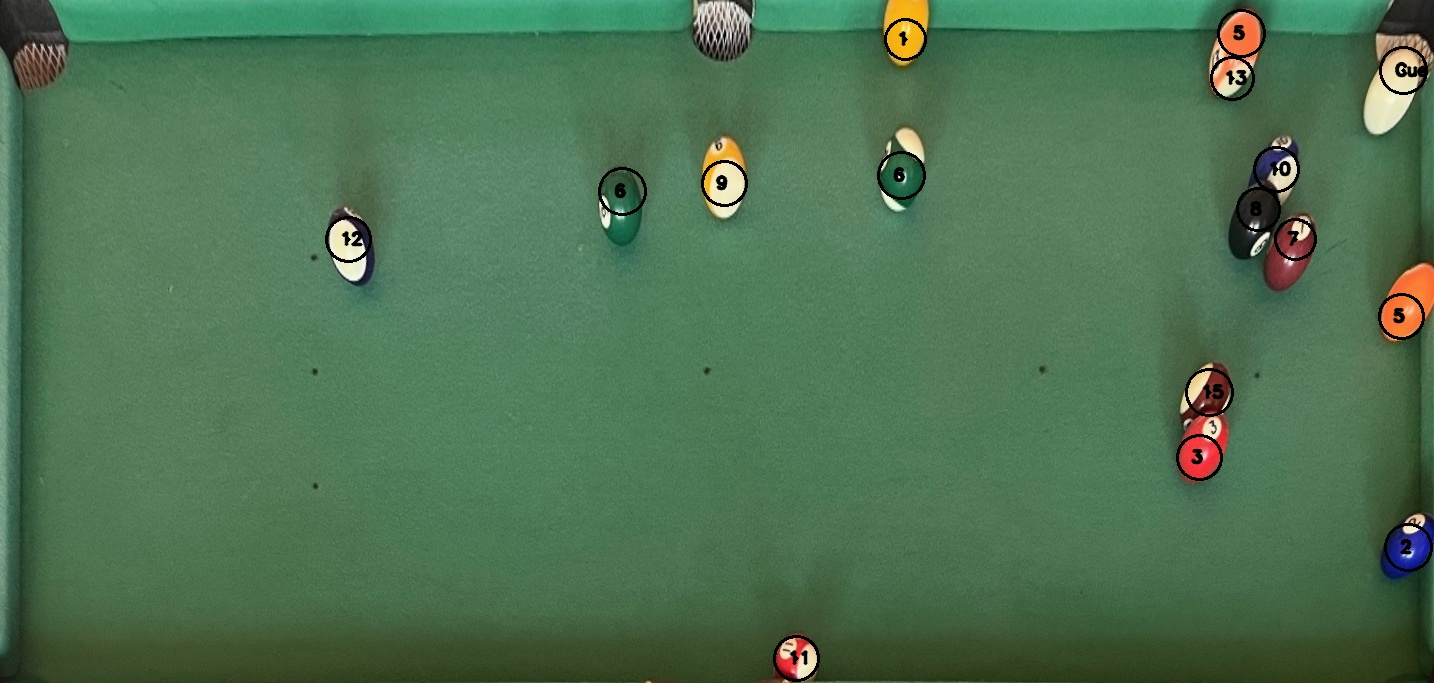
\includegraphics[width=0.85\linewidth]{report_table4_final.jpeg}
\caption{Final labelled output for Table~4; Stage~2 recognition accuracy is $92.9\%$.}
\label{fig:table4final}
\end{figure}
\vspace{2pt}

Figure~\ref{fig:table4final} shows the Table~4 output, which combines high Stage~1 recall with $92.9\%$ Stage~2 accuracy.

\subsection{Error Analysis}

After the 22-pixel cushion margin, split-mask cue gate, and raw-frame fusion, Stage~1 yields $82$ TP, $8$ FP, and $8$ FN; Stage~2 reaches $76.8\%$. I audited Table~2 because it isolates the active failures: duplicate perimeter detections, missed interior balls in the dense cluster, and rotation/specular misclassification. The cue and $9$ are resolved. Figure~\ref{fig:table2failure} shows the overlay.

\begin{figure}[H]
\centering
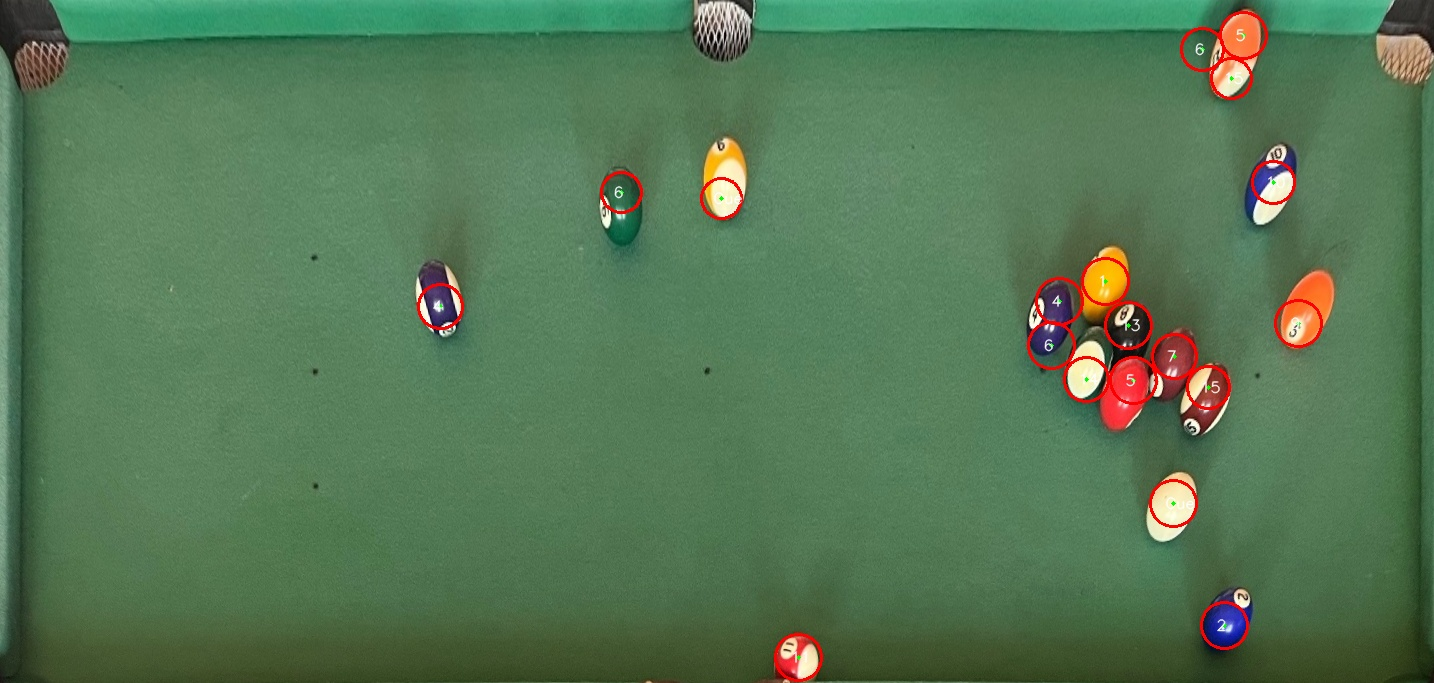
\includegraphics[width=0.92\linewidth]{table2_final.jpeg}
\caption{Final labelled output for Table 2, illustrating duplicate detections on single perimeter balls (top right) and missed detections inside dense clusters.}
\label{fig:table2failure}
\end{figure}
\vspace{2pt}

\paragraph{Failure Mode 1: Duplicate Detections on Single Balls.}
In my evaluation I observed that candidates near a table boundary can cast two accumulator peaks for the same physical ball. The cushion truncates the perimeter arc, and the two surviving arcs on opposite sides can produce centres more than $40$ pixels apart, so they lie just outside the $40$-pixel physical NMS and both survive. Figure~\ref{fig:table2failure} shows this at the top right of Table~2, where one ball receives two overlapping circles labelled $5$ and $15$. One is correct and the other is an artificial false positive; only a duplicated circular response is involved.

\paragraph{Failure Mode 2: Dense-Cluster Gradient Nullification.}
In the right-hand cluster of Table~2 I observed that touching balls break the continuous Canny arcs Hough needs. Adjacent boundaries merge into one irregular gradient, so accumulator votes spread and the interior peak stays below $param2=8.0$. Lowering the threshold admits shadow arcs, so I kept the stricter setting. This is the remaining false negative: the ball is visible but has no isolated circular evidence. A Watershed pass before circle fitting is the natural remedy.

\paragraph{Failure Mode 3: Rotation and Specular Misclassification.}
My evaluation showed that rotation and specular reflections shift 1D hue/saturation bins even when the centre is correct. A white number circle or highlight can dominate the saturation peak, while shadow can suppress the paint peak; the $30/70$ distance then lands closest to the wrong reference or exceeds $0.55$. Table~2 exposes this in its $66.7\%$ Stage~2 accuracy, where balls $3$, $8$, $12$, and $13$ receive neighbouring labels or are pulled toward the cue reference. I kept the deterministic classifier because the errors are sparse; a specular-rejection mask or rotation-invariant stripe descriptor is the next refinement.

\section{Discussion}

Final Stage~1 P/R/F1 is $0.911/0.911/0.911$; Stage~2 is $0.768$. LAB fusion was decisive: $L$ gave the silhouette while $a/b$ recovered colour boundaries in shadow; the cost was a denser edge map, which made the 40-pixel NMS and 22-pixel cushion margin necessary. The raw-frame path added three TPs without FPs, but lowering the Hough threshold alone traded precision for recall. For recognition, saturation histograms beat K-Means; the 30/70 weighting encodes the stripe effect, and the split-mask gate prevents a bullseye $9$ or $14$ from hijacking the cue. Remaining limits are duplicate perimeter responses, dense-cluster merging, and specular/stripe overlap; a spatial stripe descriptor and Watershed segmentation are the next steps.

\section{Conclusion}

I implemented a two-stage pipeline that rectifies the table, fuses LAB Canny edges, filters Hough candidates with a dynamic pocket mask and physical NMS, recovers perimeter balls through a raw-frame path, and classifies survivors with saturation-dominant histograms and a split-mask cue gate. It achieves Stage~1 P/R/F1 of $0.911$ and Stage~2 accuracy of $76.8\%$. The main residual errors are duplicate perimeter detections, dense-cluster misses, and specular/stripe confusion; Watershed segmentation and a spatial stripe descriptor are the natural next steps.

\newpage
\section*{AI Usage Statement}

Generative AI tools (Google Gemini) were used for report text revisions, LaTeX/TikZ formatting, and standalone C++ diagnostic scripts for parameter sweeps. I implemented all algorithms, selected parameters, ran experiments, and verified the reported results.

\textbf{Prompt \& Response Example 1 (Parameter Sweep Script):} \textit{User Prompt:} ``Write a diagnostic script to sweep Hough param2 from 6 to 18 and compare edge-thinned LAB maps with raw Canny maps.'' \textit{AI Response:} ``Generated a C++ benchmark logging TP/FP counts to stage2\_feature\_analysis.csv.''

\textbf{Prompt \& Response Example 2 (Gate Suggestion):} \textit{User Prompt:} ``The 1D histogram labels the 9-ball as the cue when its white circle faces the camera. How can I separate them?'' \textit{AI Response:} ``Suggested a split-mask saturation/value check comparing the 16px centre with the 21px full ball.''

\textbf{Prompt \& Response Example 3 (LaTeX Troubleshooting):} \textit{User Prompt:} ``The pipeline TikZ block wraps awkwardly and overflows the margin. How do I format a two-stage flow?'' \textit{AI Response:} ``Provided matrix/node code with explicit node distances and rounded styles.''

All core algorithmic implementations, experimental designs, parameter selections, and final data verification were conducted directly by the author.

\end{document}
